\documentclass[a4paper,12pt]{article}
%\usepackage[ngerman]{babel}
\usepackage{ucs}
\usepackage{multirow}
\usepackage{xltxtra}
\usepackage[utf8x]{inputenc}
\usepackage{fontspec}
\usepackage[automark]{scrpage2}
\usepackage{eurosym}
\usepackage{graphicx}
\usepackage[paper=a4paper,left=25mm,right=25mm,top=25mm,bottom=25mm]{geometry}
\pagestyle{scrheadings}
\setmainfont[Mapping=tex-text]{Liberation Serif}
\clearscrheadfoot
\begin{document}
\ohead{Last edit: \today}
\title{Rules Jousting Challenge 2018}

 \begin{center}

\includegraphics[width=0.5\textwidth]{logo.png}

\huge                      % Schriftgröße einstellen
\bfseries                   % Fettdruck einschalten
Rules Jousting Challenge 2018
  \end{center}
  This is only an unofficial translation. In case of any doubt, only the newest official version of the German rules will
  count. Changes in the rules since 2017 are marked in \textbf{bold}.
\section{Goal}
To design, build, and program a line following robot that can carry a knight (lightly held by 3
magnets to a steel plate) that will knock off your opponent’s knight by using it’s lance only.
\section{Who Can Play}
Teams of \emph{2 to 4 players} in one division for:
\begin{itemize}
	\item Middle School (Age 10-13)
\end{itemize}
\section{Required Materials}
Autonomous robot, any platform, costing \euro{1500} or less, and meets the following design
constraints, which will be verified during Check-In:
\begin{itemize}
\item Robot can demonstrate it is running a line following program by negotiating the jousting track
from the start point and around the curve up to the 100 point line.
\item Knights connecting structure (canning jar lid) can be attached using whatever material is
practical, method of attachment cannot provide any support to the knight, and cannot provide
any additional magnetic gripping force to aid the knight in staying attached to the structure.
\item Knight’s connecting structure is no more than 10
cm above the track \textbf{and no more than 10 cm in front of the robot}.
\item Knight’s body is completely unsupported, either by added structure or robot above the metal
plate.
\item Knight is attached to the metal plate using a special round “button” magnet.
\item No other magnets are allowed inside or outside the robot.
\item A sensor must be used to detect an follow the line.
\item During the competition, the official knight of this year must be used. Knights, magnets, jar lids and lances will be available a the track.
\item Volume of the robot must not exceed 65030 cubic cm.
\end{itemize}
\section{General Rules of Play}
\begin{itemize}
	\item A line following program must control your robot’s motion.
	\item During a jousting match, up to 5 attempts will be allowed to knock your opponent’s knight off.
	\item If five (5) passes are used and no knight is knocked off, the joust will be considered a DRAW.
	\item If both knights fall, the LAST knight to hit the floor, as determined by the track official, will be
	awarded the win.
	\item \textbf{Only the lance can knock the knight off; if the knight is knocked off something other than the
		lance, then continue with the next pass.}
	\item ONLY the lance may cross the midline of the track (\textasciitilde 13 cm from either of the 2 parallel lines).
	\item \textbf{The number of points decreases by 10 \% after any pass.}
\end{itemize}
\section{Challenge Specifications}
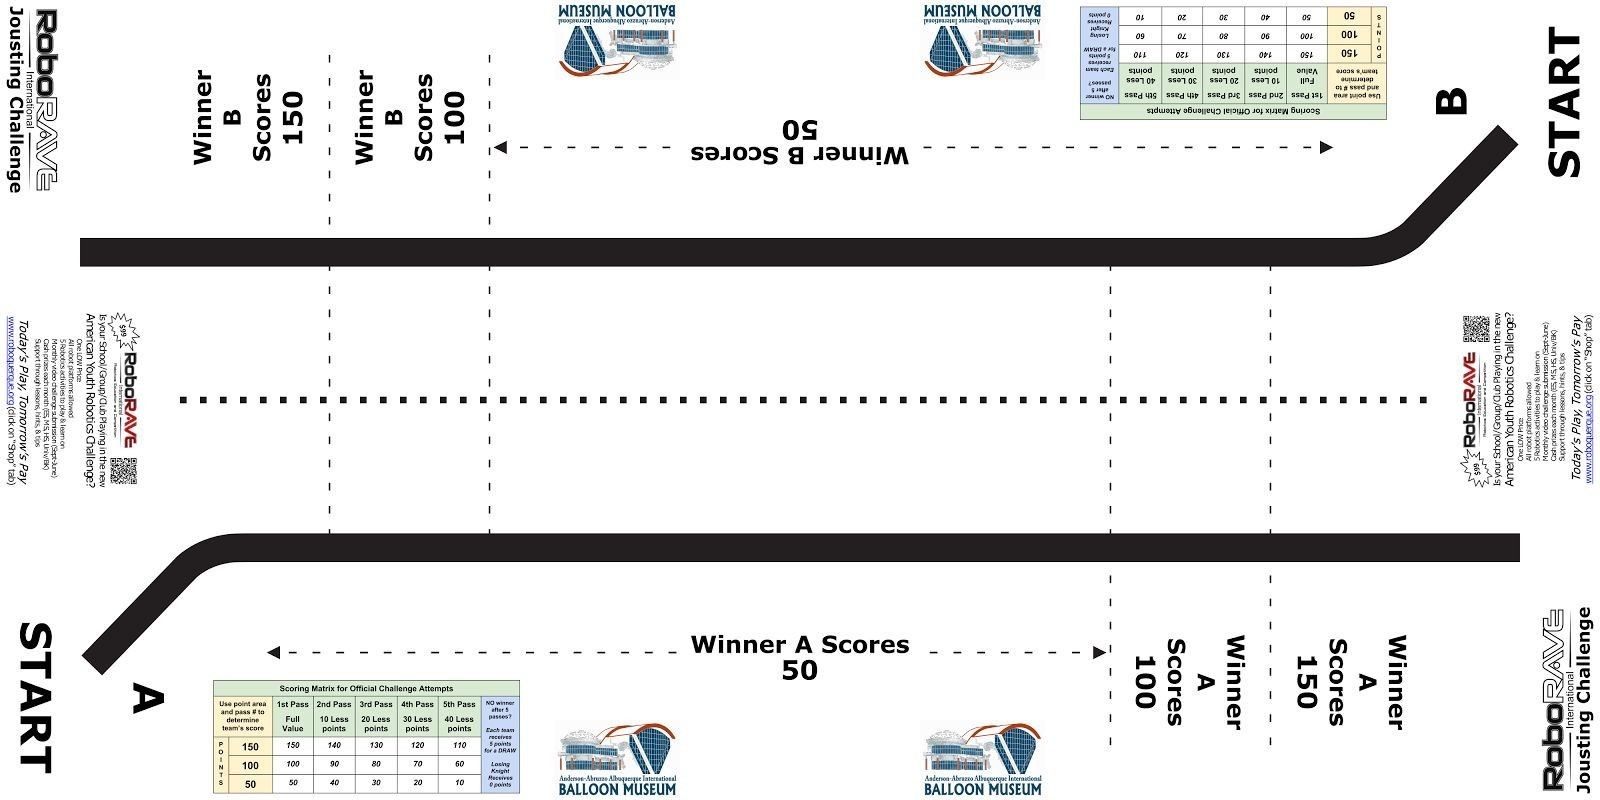
\includegraphics[width=1\textwidth]{track.png}
\begin{itemize}
	\item Two (2) parallel, \textasciitilde2.5 cm wide black lines on a white PVC vinyl track.
	\item Each line has a slight curve at the start.
	\item A meter stick will be inserted under the track the length of the midline to create a “wall”.
	\item Three scoring zones: 150 points (0.0 cm to \textasciitilde15 cm from start); 100 points (\textasciitilde15 cm to \textasciitilde30 cm
	from start); 50 points (\textasciitilde30 cm to \textasciitilde91 cm from start).
\end{itemize}
\section{Scoring Period}
\par The way the earned points are counted for the challenge will be announced on the first day of the event. Scoring will likely be in form of a tournament.
\section{Scoring}
\begin{itemize}
\item Full score is awarded ONLY if you knock your opponent off during the 1 st of 5 attempts. Each successive attempt used decreases the point value. See matrix below.
wird.
\item Higher scores are earned by knocking your opponent off closer to their START position.
\item If the knight (not the lance) is lying within two point areas, the higher point value is awarded.
\item Pass - an attempt is made by both robots to knock each other off, but NO
ONE does
\item Each team has 5 Passes to knock their opponent OFF.
\item 5 passes,
no
winner?
Draw -
each
team gets
5 points
\end{itemize}
\section{Scoring matrix}
\begin{center}
\begin{tabular}{|c|c|c|c|c|c|} \hline
	\multirow{2}*{Area} & 1st Pass & 2nd Pass & 3rd Pass & 4th Pass & 5th Pass \\
	 & 100\% & 90\% & 80\% & 70\% & 60\% \\ \hline
	150 & 150 & \textbf{135} & \textbf{120} & \textbf{105} & \textbf{90} \\ \hline
	100 & 100 & 90 & 80 & 70 & 60 \\ \hline
	50 & 50 & \textbf{45} & \textbf{40} & \textbf{35} & \textbf{30} \\ \hline
\end{tabular}
\end{center}
\end{document}